\chapter{Uppaal Modelling}
In the scope of this mini project we only choose to model some specific parts of the previously described steps.
Moreover, we do so in a slightly simplified manner.

The aspects we want to model are:
\begin{enumerate*}[label=\itshape\arabic*\upshape)]
    \item The process of joining the network;
    \item transmitting and receiving playback commands; and
    \item periodically synchronizing the slaves.
\end{enumerate*}
These roughly translates to~\cref{itm:connect},~\cref{itm:txrx}, and~\cref{itm:sync} from the aforementioned list of steps in the \textit{Introduction}.

\bigskip
To simplify the model and modelling process, we have some assumptions about the system, which does not reflect reality fully.
These are:
\begin{enumerate}[label=\itshape\arabic*\upshape)]
    \item All slaves will eventually try to connect to the master.
    \item The master cannot listen for incoming connection requests, while transmitting commands to devices already connected.
    \item Audio data, and the transmission or receiving of audio data, will not be considered in the model.
    \item The master transmits commands to the slaves sequentially, i.e.\ to one slave at a time.
    \item All slaves connected to the master will always receive transmitted commands.
    \item Synchronization of the slaves, is represented by a local boolean called \texttt{in\_sync}.
\end{enumerate}

Our system consists of two templates, one for the \textit{master} device and one for a \textit{slave}.
The system is instantiated with one master and five slaves.
In the following two sections we present the templates for the master and slave.

\section{Master Device}
The master device is the one which drives the system per say, and a system can only contain one master.

In~\cref{fig:master_model} the master model template can be seen.
The template consists of four color coded \enquote{zones}, the initial location, and a location named \texttt{main\_idle}.

\begin{description}
    \item[\textcolor{orange}{The Orange Zone}] \hfill\\
        Represents the locations related to listening for slaves, which are trying to connect.
        The master will enter this zone when a slave request to join the network.
        The master will then either send a confirmation to the slave, or timeout and return to the \texttt{main\_idle} location.
    \item[\textcolor{cyan}{The Cyan Zone}] \hfill\\
        This zone consists of a single location in the model, where the decision of whether it is time to send synchronization command, or a playback command.
        The synchronization command will be chosen if a local clock called \texttt{sync\_timer} is greater than or equal to a constant called \texttt{sync\_delay}.
        The \texttt{sync\_timer} is only reset when the master sends synchronization commands to all connected slaves.
    \item[\textcolor{blue}{The Blue Zone}] \hfill\\
        To reach all connected slaves with commands, the master must transmit then sequentially --- one command to one slave at a time.
        Because of this behaviour, the blue zone represents a loop which is iterated through one time for each connected slave.
        Each iteration broadcasts on a channel, related to a specific command and slave.
        At the first iteration, the variable \texttt{msg\_type} is changed to ensure that the same command is transmitted to all slaves.
        Finally, \texttt{msg\_type} is reset to allow for a different command to be send.
    \item[\textcolor{magenta}{The Magenta Zone}] \hfill\\
        The synchronization command is slightly different from the playback commands, in that it must be transmitted once every \texttt{sync\_delay}.
        To convey this difference in the model we use a different zone which solely deals with transmitting synchronization commands to all connected slaves.
\end{description}

\begin{figure}[htb]
    \centering
    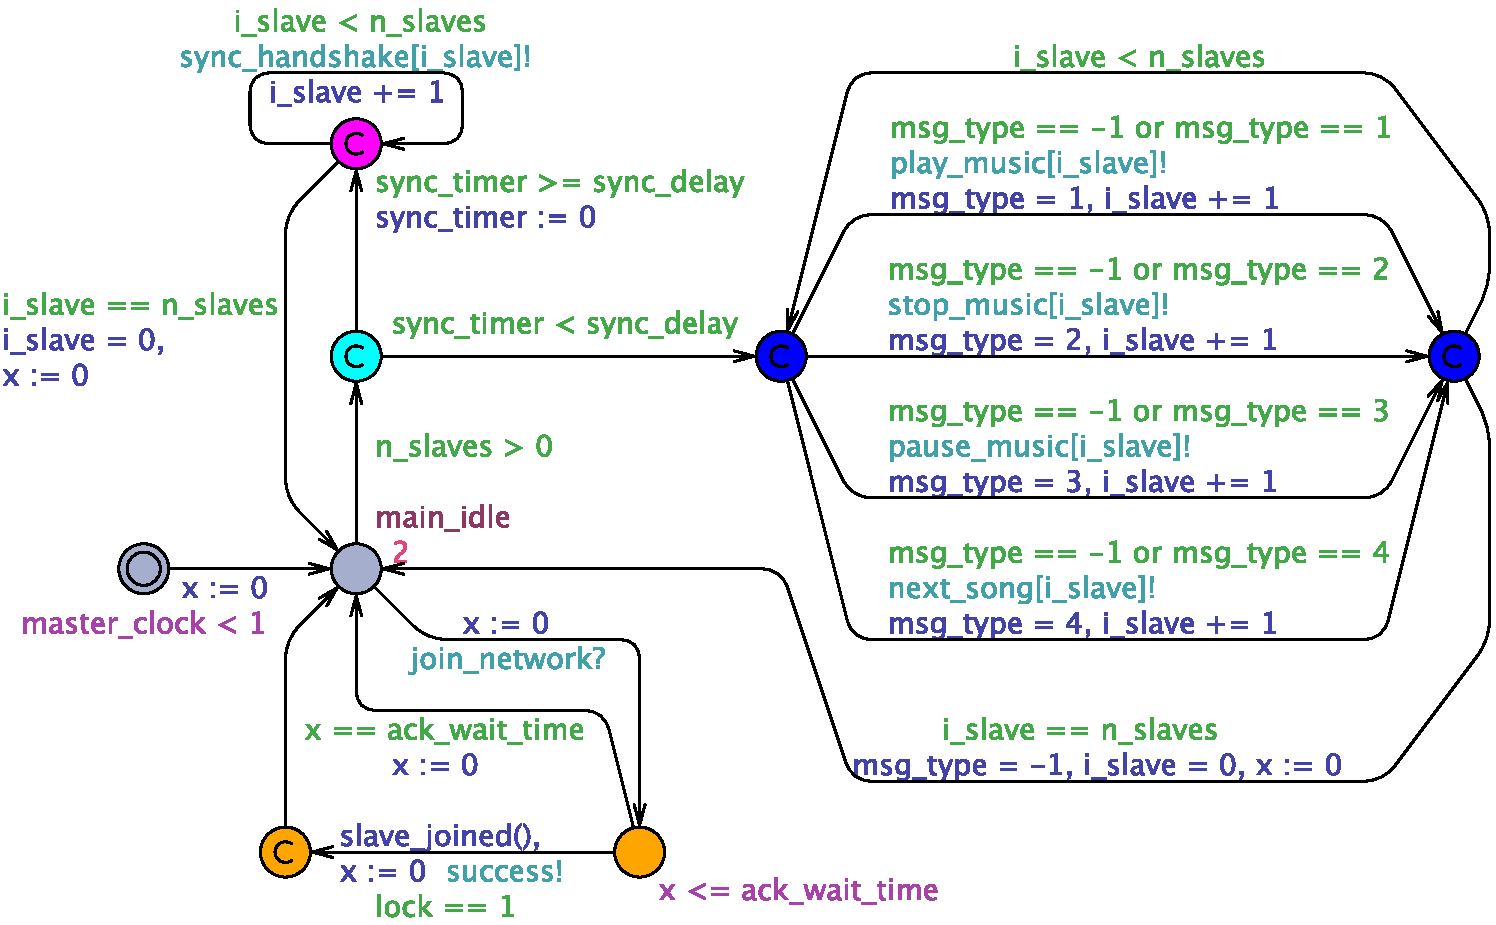
\includegraphics[width=1\textwidth]{master_model.pdf}
    \caption{Model of the \textit{master} device}\label{fig:master_model}
\end{figure}

Maybe more content about master model.

\section{Slave Device}

In the context of our system, the \textit{slave} is more passive, in that after having joined the \textit{master} it only receives commands.
However, to represent the local synchronization being able to drift, we use a Uppaal SMC construct where the slaves have a $\frac{1}{1000}$ risk of drifting out of sync.

Additionally to being able to drift out of sync, the slave needs to receive an acknowledgement from the master, when trying to join the network.

\bigskip
As with the template of the master, presented in the previous section, the slave template contains four colored zones.
All of which roughly corresponds to the same colored zones in the master template.
The template can be seen in~\cref{fig:slave_model}.
The four zoned are described as follows:

\begin{description}
    \item[\textcolor{orange}{The Orange Zone}] \hfill\\
        For the slave to join the network of the master, it must first request to join, and then wait for an acknowledgement.
        If this acknowledgement is not received within a given time (\texttt{ack\_wait\_time}) the slave will fail to join, and retry at a later time.
    \item[\textcolor{cyan}{The Cyan Zone}] \hfill\\
        This zone is where the slave listens for commands from the master.
        However, while in this zone, the slave may drift out of sync as previously described.
    \item[\textcolor{blue}{The Blue Zone}] \hfill\\
        Here the slave receives playback commands from the master, via a broadcast channel.
    \item[\textcolor{magenta}{The Magenta Zone}] \hfill\\
        This is where the slave receives the synchronization command from the master, and acts on it by setting its local \texttt{in\_sync} boolean to true.
\end{description}

\begin{figure}[htb]
    \centering
    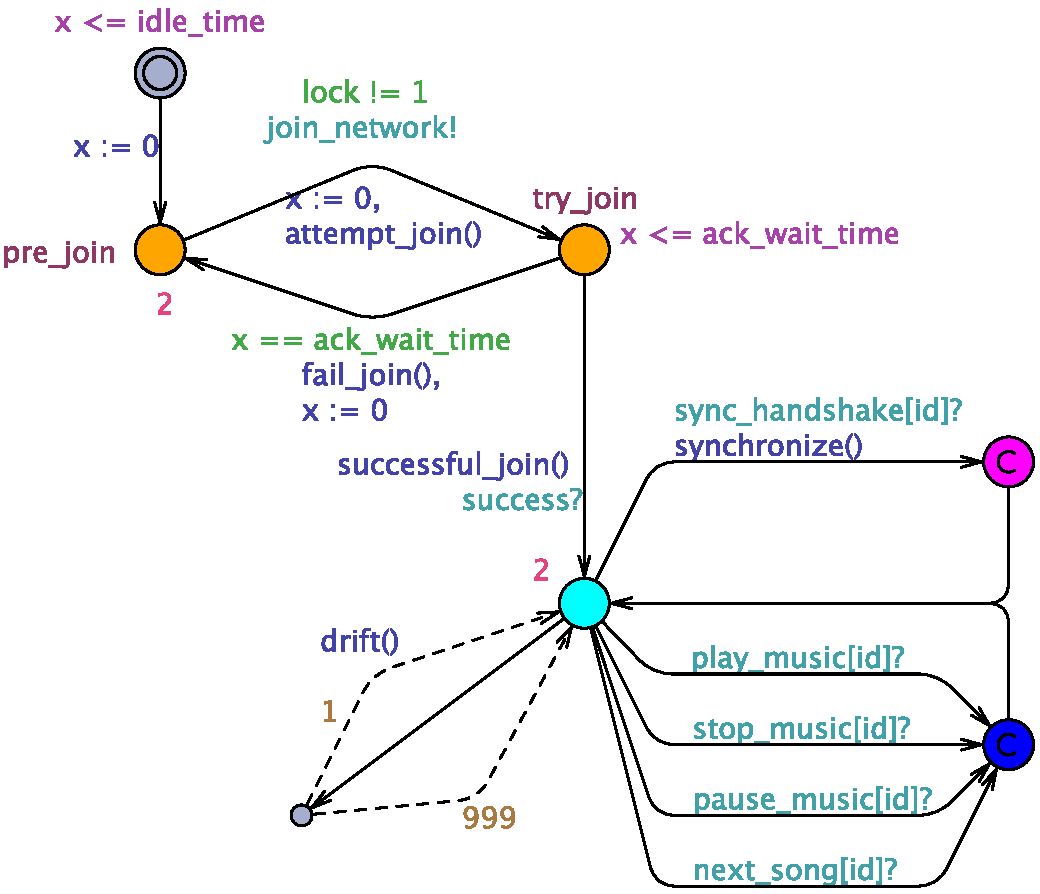
\includegraphics[width=0.7\textwidth]{slave_model.pdf}
    \caption{Model of a \textit{slave} device}\label{fig:slave_model}
\end{figure}

